\vspace{-0.5em}
In this section, we focus on linear models.
We have labeled data points $(\a_1, b_1), (\a_2, b_2), \ldots, (\a_K, b_K) \in \R^n \times \R$, and our goal is to minimize the function
\[
f(\x) = \frac{1}{K} \sum_{k = 1}^K \| \a_k^\top \x - b_k \|_2^2 \; ,
\]
i.e., minimize the empirical least squares loss.
The full-precision SGD works as 
follows: at step $\x_k$, our gradient estimator is $\g_k^{(full)} = \a_{\pi(k)} (\a_{\pi(k)}^\top \x - b_{\pi(k)})$, where $\pi(k)$ is a uniformly random integer from $1$ to $K$.
We abuse the notation and let $\a_k = \a_{\pi(k)}$.
We have $\E [\g_k^{(full)}] = \nabla f(\x_k)$.

\vspace{-1em}
\paragraph*{Stochastic Quantization} 
Given a vector
$\v$, let $M(\v)$ be a scaling factor such that
$-1 \le \v/M(\v) \le 1$. Without loss of generality,
let $M(\v)=||\v||_2$. We partition
the interval $[-1, 1]$ using $s+1$ separators:
$-1 = l_0 \le l_1 ... \le l_{s} = 1$; for
each number $v$ in $\v/M(\v)$, we 
quantize it to one of two nearest 
separators: $l_i \le v \le l_{i+1}$. 
We denote the \emph{stochastic quantization} function by $Q(\v, s)$
and choose the probability of quantizing to
different separators such that $\E[Q(\v, s)] = \v$.
We use $Q(\v)$ when $s$ is not relevant.
We assume that these
separators are uniformly distributed,
and revisit this in Section~\ref{sec:optimal}.
We have~\cite{Alistarh:2016:ArXiv}: 
\begin{lemma}
\label{lem:quant-facts}
For any vector $\vec{v} \in \R^n$, we have that $\E [Q (\vec{v},s)] = \vec{v}$, and furthermore, we have
$
\E [\| Q (\vec{v},s) \|_2^2] \leq (1 + \min( n/s^2,\sqrt{n}/s)) \| \vec{v} \|_2^2 \; .
$
\end{lemma} 




\vspace{-0.5em}
\subsection{Naive Stochastic Quantization is Biased}

\vspace{-0.5em}
We focus on quantizing the input samples.
We first establish that, when we quantize $\a_k$
using the stochastic quantization methods designed
for gradient, it introduces significant bias.
Let $\hat{\a_k} = Q(\a_k)$ be the quantized
sample, the gradient becomes
\[
\g_k := \hat{\a_k} \hat{\a_k}^\top \x - \hat{\a_k} b_k.
\]
It is not hard to see that the expected gradient is: 
\[
\E[\g_k] := \a_k \a_k^\top \x - \a_k b_k + D_{\a} \x, 
\]
where $D_{\a}$ is diagonal and its $i$th diagonal element is 
\[
\E[ Q(\a_i)^2 ] - \a_i^2.
\]

%\todo{y axis here is weird}
\begin{wrapfigure}{r}{0.23\textwidth}
  \begin{center}
    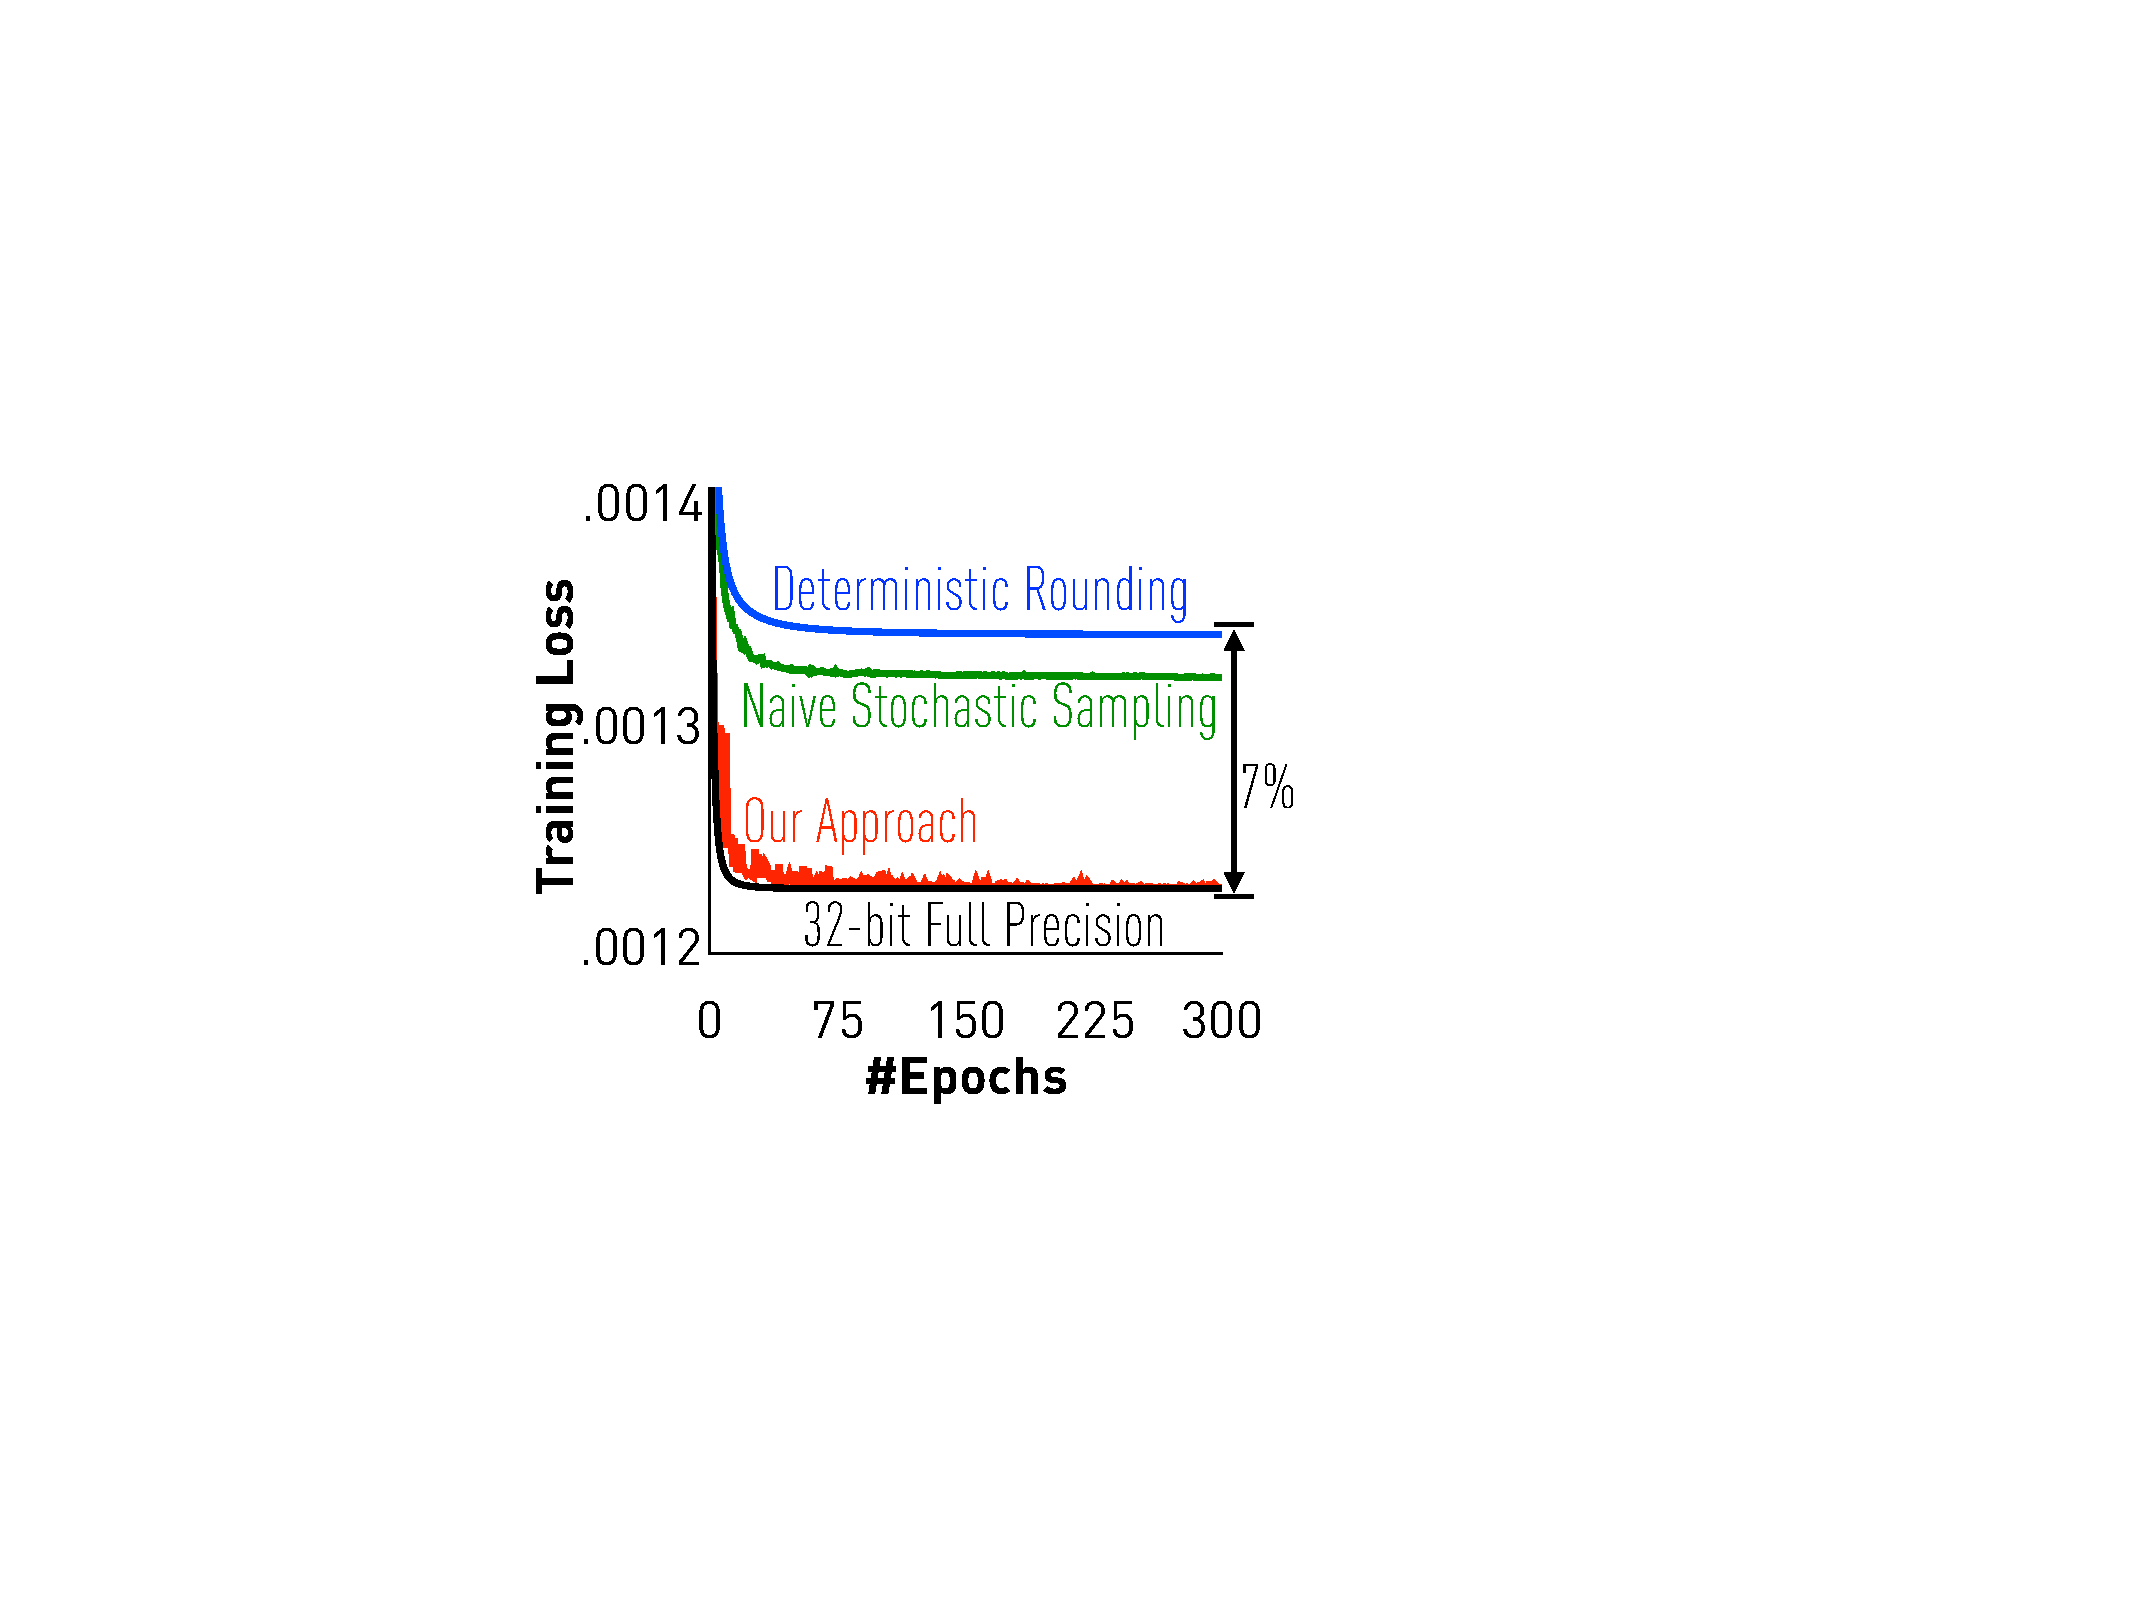
\includegraphics[width=0.23\textwidth]{micro-experiments/gap.pdf}
  \end{center}
  \label{fig:gap}
\end{wrapfigure}

\vspace{-0.5em}
Since $D_{\a}$ is non-zero, we obtain a \emph{biased} estimator of the gradient, so the iteration is unlikely to converge. 
The figure on the right illustrates the bias
caused by a non-zero $D_{\a}$.
In fact, it is easy to see that in instances where the minimizer $\x$ is large and gradients become small, we will simply diverge. 

\vspace{-0.5em}
\subsection{Double Sampling}
\vspace{-0.5em}

We now present a simple method to fix the biased gradient estimator.
We generate two independent
random quantizations and revise the gradient:
\[
\g_k := Q_1 (\a_k) (Q_2 (\a_k)^\top \x + b_k) \; .
\]
This gives us an unbiased estimator 
of the gradient.

\vspace{-0.5em}
\paragraph{Variance}

Let $r = r(s) = 1 + \min (n / s^2, \sqrt{n}/ s)$ be the blow-up in the second moment because of quantization:
\begin{lemma}
\label{lem:qbound}
    Given $\a_k, \x, b_k$, suppose $\| \a_k \|_2^2 \leq A^2, \| \x \|_2^2 \leq R^2$ and $\max_i |\a_k| \leq M_a$.
    Let $\g_k^{(full)}$ be the unquantized stochastic gradient. We have
    \[
    \E_{Q_1, Q_2} [\| \g_k \|_2^2] \leq r \cdot \left( \| \g_k^{(full)} \|_2^2 \cdot \frac{M_a^2}{\| \a_k \|_2^2} + \frac{A^2 M_a^2 R^2}{s^2} \right)\; .
    \]
\end{lemma}

This implies the following variance bound:
\begin{corollary}
    Let $\a_k, \x, b_k, \g_k^{(full)}$ be as above.
    Suppose $\E [\| \g_k^{(full)} - \nabla f(\x_k) \|_2^2 ] \leq \sigma^2$ and $\E [\| \g_k^{(full)} \|_2^2] \leq B$. We have
    \[
    \E \left[ \| \g_k - \nabla f(\x_k) \|_2^2 \right] \leq  \sigma^2 + \left(r \frac{M_a^2}{\| \a_k \|_2^2} - 1\right) B + \frac{r A^2 M_a^2 R^2}{s^2} \; ,
    \]
    where the expectation is taken over $\g_k^{(full)}$ and the randomness of the quantization.
\end{corollary}

This corollary suggests that the quantized stochastic gradient variance is bounded by
\[
\E \left[ \| \g_k - \nabla f(\x_k) \|_2^2 \right] \leq \sigma^2 + \Theta(n/s^2) \;
\]
in the scenario when $M_i (\vec{v}) = \| \vec{v} \|_2 $.
The first term $\sigma^2$ is introduced by stochastic gradient, while the second term is introduced by quantization. Because the value of $s$ is 
exponential to the number of bits, to ensure these two terms are comparable (to maintain the same convergence rate), the number of bits needs to be greater than $\Theta(\log n / \sigma)$. We see that even for linear models with millions
of features, 32-bits is likely to be  ``overkill.''

\vspace{-0.5em}
\paragraph*{Overhead of Storing Two Samples}
One system implication of double sampling is the overhead of sending
two samples instead of one. We note that this will not introduce $2\times$
overhead in terms of data communication, instead, just a single more bit
for the second sample because of the correlation (these two samples 
are only different by at most one bit). More generally, because samples
are used symmetrically, sending $k$ samples only require $\log_2 k$ more bits.

\vspace{-0.5em}
\paragraph*{Extensions}

All of our results can be applied to 
 problems 
with possibly non-smooth regularization term. The key substitution is to use the proximal update defined in \eqref{eq:proxupdate}.
Also, extending our result to least-squares SVMs for classification is trivial~\cite{Suykens:1999:Book}.
We leave these details to the full version
of this paper.

\vspace{-0.5em}
\subsection{End-to-end Quantization}
\vspace{-0.5em}

We can now develop an end-to-end quantization strategy that
quantizes gradients, model, and input samples all 
at the same time. The gradient becomes:
\[
\g_k := Q_1 \left( Q_2(\a_k, s ) ( Q_3(\a_k, s)^\top Q_4(\x, s) + b_k) , s \right),
\]
\noindent 
where all $Q$'s are independent quantizations.

%  $Q_3$ and 
%The iteration becomes: 
%
%\begin{eqnarray}
%	\x = \x - \gamma \g_k.
%\end{eqnarray}

\noindent From combining the previous results, we have:

\begin{corollary}
    \label{cor:full-quantization}
    Let $\a_k, \x, b_k$ be so that $\| \a_k \|_2^2 \leq 1, \| \x \|_2^2 \leq R^2$.
    Let $M_a, M_x$ be as above, and let $\g_k^{(full)}$ be the (unquantized) stochastic gradient.
    We have
    \[
    \E [\| \g_k \|_2^2] \leq r^2 M_a \cdot \left(  \| \g_k^{(full)} \|_2^2 + \frac{R^2}{s^2}   + \frac{r M_a R^2}{s^2} \right) \; .
    \]
\end{corollary}